\documentclass{article}
\usepackage[utf8]{inputenc}
\usepackage[french]{babel}
\usepackage[margin=2cm]{geometry}
\usepackage{multicol}
\usepackage{graphicx}
\usepackage{float}
\usepackage{adjustbox}

\title{Étiquetage morpho-syntaxique avec un perceptron: \\
  \large j'aime les bananes salées}

\date{13 avril 2019}
\author{Adrien Chesneau et Julien Guyot}

\begin{document}

\maketitle
\section{Introduction}
Ce projet porte sur
l'étiquetage morpho-syntaxique, dit Part of Speach, d'un
corpus.

\subsection{Part of speech}
L'étiquetage morpho-syntaxique est l'association à chaque mot d'un
texte des informations grammaticales liées à ce même mot.


Dans le cadre de ce projet, les informations grammaticales se limitent
aux informations liés à la nature grammaticale des mots. Les natures
possibles sont les suivantes: 


\begin{description} 
\item[ADJ] Les adjectifs qui caractérisent le nom et s'accordant en genres et en nombres. 
\item[ADV] Les adverbes qui précisent le sens d'un verbe et marque le degré d'intensité de la phrase. 
\item[INTJ] Les interjections qui montrent l'exclammation. 
\item[NOUN] Les noms qui désignent une réalité concrète ou abstraite et s'accordant en genres et en nombres. 
\item[PROPN] Les noms propres qui désignent le nom d'un individu, un lieu ou un objet spécifique. 
\item[VERB] Les verbes qui est les noyaux de la phrase, ils expriment un état ou une action et varient en personne. 
\item[DET] Les déterminants précèdent un nom et qui marque le genre et le nombre de celui-ci. 
\item[NUM] Les chiffres qui expriment un nombre et une relation avec un nombre. 
\item[PRON] Les pronoms qui désignent une personne et remplacent un élément déjà nommé. 
\item[CCONJ] Les conjonctions de coordinations qui permettent de relier deux mots, propositions et phrases. 
\item[AUX] Les auxiliaires qui sont des verbes qui se combinent à un verbe principale afin de constituer un temps composé, expriment le temps, le mode et la voix. 
\item[ADP] Les prépositions qui permettent de relier un nom, verbe ou adjectif à un nom, pronom, adverbe ou à un verbe. 
\item[SCONJ] Les conjonctions de subordinations permettant d'introduire une proposition subordonnée. 
\item[PART] Les particules qui permettent de donner un sens une fois associés à un mot. 
\item[PUNCT] Les ponctuations qui permettent l'organisation de l'écrit en indiquant les pauses et intonations ou en précisant le sens de la phrase. 
\item[SYM] Les symboles qui sont des mots spéciaux différants des mots ordinaires par leurs formes, fonctions ou les deux. 
\item[X] Les autres qui sont des mots ne pouvant être assignés aux autres classes grammaticales. 
\end{description}


\subsection{Objectif}
Notre objectif est d'implémenter et d'entraîner
un neurone artificiel afin de prédire
la nature de chaque mot, connaissant son contexte
(égal à la phrase dans lequel il se trouve).


Pour cela, nous disposons de plusieurs jeux de données provenant pour
la plupart de la base \emph{ Universal Dependencies }. Nous avons
écarté les \emph{dataset} en anglais pour nous concentrer sur les
données écrites en Français. Ces données seront décrites plus en
détail dans la deuxième partie.


\subsection{Plan}
Dans un premier temps, nous allons décrire les données, et montrer
quelques informations sur ces dernières. \\
Ensuite, nous présenterons la structure et le contenu du code, ainsi
que les perceptrons et la modélisation choisie \\
Nous montrerons et expliquerons les résultats obtenus,
avant de conclure.


%Grâce à ces données, nous avons voulu créer un perceptron utilisant
%différents modèles pouvant prédire l'étiquetage morpho-syntaxique des
%mots dans les  phrases. Nous avons aussi voulu construire plusieurs
%fonctions d'analyses afin d'étudier les données à notre dispositions. 


\section{Présentation des données}
Comme dit précédemment, nous avons à disposition plusieurs sets de
données en anglais et en français. Nous utiliserons uniquement les
sets de données en français.


Ces données sont sous forme de fichiers {\verb .json }, chaque
fichier correspond à un \emph{ dataset }, qui est un ensemble de
couples (phrase, labels), ou chaque label $\in$ labels correspond à la
nature grammatical du mot correspondant.


Pour chaque set de données, nous indiquons les informations suivantes: 
\begin{description}
\item[Présentation brève du dataset]
\item[Pourcentage des mots hors vocabulaire] Pourcentage de mots
  apparaissant uniquement dans les données de test, et pas dans les
  données d'entraînement
\item[KL-Divergence] La divergence de Kullback-Leibler entre les
  données d'entraînement et de test
\item[Distribution des différents labels] dans le dataset
\item[Mots les plus utilisés] dans le dataset. 
\end{description}

\singlespacing
\clearpage \subsection{pud} 
 \begin{itemize} 
 \item[Présentation :] Phrases qui proviennent de sites informatifs, id est de journaux ou de Wikipedia

 \item[Pourcentage de mots hors vocabulaire : ]54.04
 \item[KL-Divergence :]0.256
 \end{itemize}  \subparagraph{Données de test \\ }  
 Nombre de phrases : 1000\\ 
\begin{figure}[H] \begin{minipage}{0.48\textwidth} \centering \begin{tabular}{|l || *{11 }{|c} |} \hline
Mot & Apparitions  \\ \hline
\begin{verb} , \end{verb} &1178\\ \hline
\begin{verb} de \end{verb} &1175\\ \hline
\begin{verb} . \end{verb} &985\\ \hline
\begin{verb} la \end{verb} &675\\ \hline
\begin{verb} et \end{verb} &442\\ \hline
\begin{verb} le \end{verb} &414\\ \hline
\begin{verb} les \end{verb} &399\\ \hline
\begin{verb} à \end{verb} &370\\ \hline
\begin{verb} l' \end{verb} &328\\ \hline
\begin{verb} des \end{verb} &327\\ \hline

\end{tabular}
\caption{ Mots les plus utilisés dans le set pud(test) } \label{Fig:muw}\end{minipage} 
\begin{minipage}{0.48\textwidth} \centering
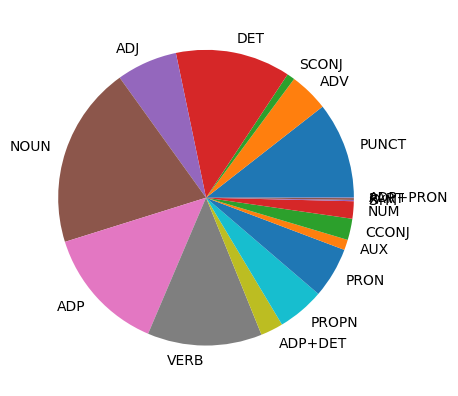
\includegraphics[width=.7\linewidth]{pudtest_img.png}
\caption{distribution des labels}
\end{minipage}
\end{figure} \subparagraph{Données de train \\ }  
 Nombre de phrases : 803\\ 
\begin{figure}[H] \begin{minipage}{0.48\textwidth} \centering \begin{tabular}{|l || *{11 }{|c} |} \hline
Mot & Apparitions  \\ \hline
\begin{verb} de \end{verb} &1114\\ \hline
\begin{verb} , \end{verb} &1016\\ \hline
\begin{verb} . \end{verb} &750\\ \hline
\begin{verb} la \end{verb} &683\\ \hline
\begin{verb} et \end{verb} &544\\ \hline
\begin{verb} l' \end{verb} &486\\ \hline
\begin{verb} des \end{verb} &432\\ \hline
\begin{verb} à \end{verb} &404\\ \hline
\begin{verb} d' \end{verb} &397\\ \hline
\begin{verb} le \end{verb} &385\\ \hline

\end{tabular}
\caption{ Mots les plus utilisés dans le set pud(train) } \label{Fig:muw}\end{minipage} 
\begin{minipage}{0.48\textwidth} \centering
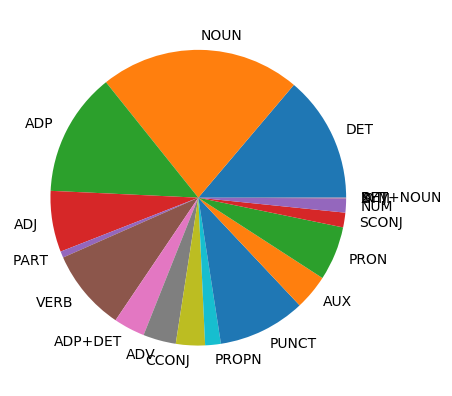
\includegraphics[width=.7\linewidth]{pudtrain_img.png}
\caption{distribution des labels}
\end{minipage}
\end{figure}


\clearpage \subsection{ftb } 
 \begin{itemize} 
 \item[Présentation :] Phrases provenant du journal «Le Monde»

 \item[Pourcentage de mots hors vocabulaire : ]7.099
 \item[KL-Divergence :]0.110
 \end{itemize}  \subparagraph{Données de test \\ }  
 Nombre de phrases : 2541\\ 
\begin{figure}[H] \begin{minipage}{0.48\textwidth} \centering \begin{tabular}{|l || *{11 }{|c} |} \hline
Mot & Apparitions  \\ \hline
\begin{verb} , \end{verb} &4528\\ \hline
\begin{verb} de \end{verb} &3593\\ \hline
\begin{verb} . \end{verb} &2258\\ \hline
\begin{verb} __DIGIT__ \end{verb} &2200\\ \hline
\begin{verb} la \end{verb} &2016\\ \hline
\begin{verb} l' \end{verb} &1350\\ \hline
\begin{verb} à \end{verb} &1333\\ \hline
\begin{verb} le \end{verb} &1293\\ \hline
\begin{verb} des \end{verb} &1255\\ \hline
\begin{verb} les \end{verb} &1222\\ \hline

\end{tabular}
\caption{ Mots les plus utilisés dans le set ftb(test) } \label{Fig:muw}\end{minipage} 
\begin{minipage}{0.48\textwidth} \centering
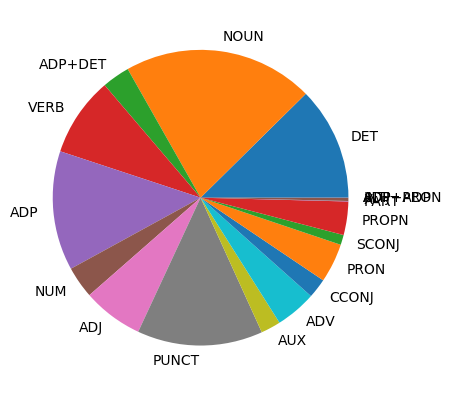
\includegraphics[width=.7\linewidth]{ftbtest_img.png}
\caption{distribution des labels}
\end{minipage}
\end{figure} \subparagraph{Données de train \\ }  
 Nombre de phrases : 14759\\ 
\begin{figure}[H] \begin{minipage}{0.48\textwidth} \centering \begin{tabular}{|l || *{11 }{|c} |} \hline
Mot & Apparitions  \\ \hline
\begin{verb} , \end{verb} &27318\\ \hline
\begin{verb} de \end{verb} &22518\\ \hline
\begin{verb} . \end{verb} &13735\\ \hline
\begin{verb} __DIGIT__ \end{verb} &11104\\ \hline
\begin{verb} la \end{verb} &10780\\ \hline
\begin{verb} l' \end{verb} &8129\\ \hline
\begin{verb} à \end{verb} &7984\\ \hline
\begin{verb} le \end{verb} &7255\\ \hline
\begin{verb} les \end{verb} &7086\\ \hline
\begin{verb} des \end{verb} &7071\\ \hline

\end{tabular}
\caption{ Mots les plus utilisés dans le set ftb(train) } \label{Fig:muw}\end{minipage} 
\begin{minipage}{0.48\textwidth} \centering
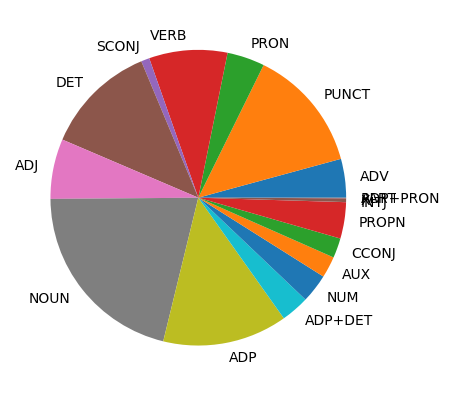
\includegraphics[width=.7\linewidth]{ftbtrain_img.png}
\caption{distribution des labels}
\end{minipage}
\end{figure}


\clearpage \subsection{spoken } 
 \begin{itemize} 
 \item[Présentation :] Données sur le français oral

 \item[Pourcentage de mots hors vocabulaire : ]32.14
 \item[KL-Divergence :]0.366
 \end{itemize}  \subparagraph{Données de test \\ }  
 Nombre de phrases : 726\\ 
\begin{figure}[H] \begin{minipage}{0.48\textwidth} \centering \begin{tabular}{|l || *{11 }{|c} |} \hline
Mot & Apparitions  \\ \hline
\begin{verb} de \end{verb} &380\\ \hline
\begin{verb} est \end{verb} &262\\ \hline
\begin{verb} euh \end{verb} &222\\ \hline
\begin{verb} la \end{verb} &219\\ \hline
\begin{verb} et \end{verb} &193\\ \hline
\begin{verb} que \end{verb} &188\\ \hline
\begin{verb} le \end{verb} &181\\ \hline
\begin{verb} l' \end{verb} &177\\ \hline
\begin{verb} à \end{verb} &169\\ \hline
\begin{verb} je \end{verb} &162\\ \hline

\end{tabular}
\caption{ Mots les plus utilisés dans le set spoken(test) } \label{Fig:muw}\end{minipage} 
\begin{minipage}{0.48\textwidth} \centering
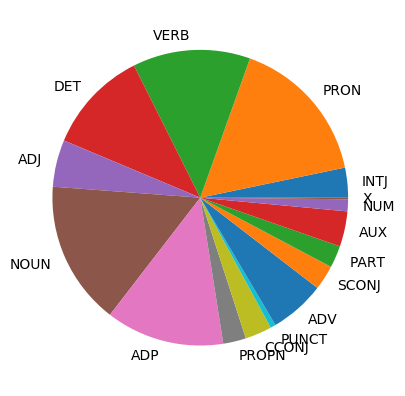
\includegraphics[width=.7\linewidth]{spokentest_img.png}
\caption{distribution des labels}
\end{minipage}
\end{figure} \subparagraph{Données de train \\ }  
 Nombre de phrases : 1153\\ 
\begin{figure}[H] \begin{minipage}{0.48\textwidth} \centering \begin{tabular}{|l || *{11 }{|c} |} \hline
Mot & Apparitions  \\ \hline
\begin{verb} de \end{verb} &529\\ \hline
\begin{verb} euh \end{verb} &489\\ \hline
\begin{verb} est \end{verb} &362\\ \hline
\begin{verb} la \end{verb} &339\\ \hline
\begin{verb} et \end{verb} &328\\ \hline
\begin{verb} le \end{verb} &294\\ \hline
\begin{verb} à \end{verb} &282\\ \hline
\begin{verb} c' \end{verb} &264\\ \hline
\begin{verb} je \end{verb} &223\\ \hline
\begin{verb} qui \end{verb} &218\\ \hline

\end{tabular}
\caption{ Mots les plus utilisés dans le set spoken(train) } \label{Fig:muw}\end{minipage} 
\begin{minipage}{0.48\textwidth} \centering
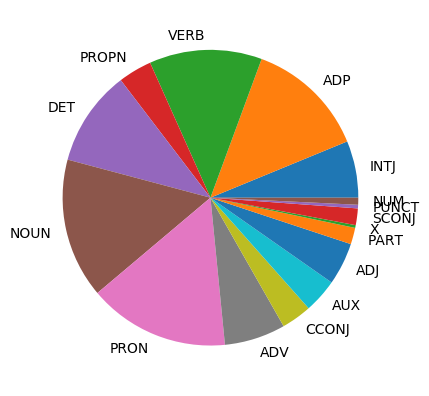
\includegraphics[width=.7\linewidth]{spokentrain_img.png}
\caption{distribution des labels}
\end{minipage}
\end{figure}


\clearpage \subsection{sequoia } 
 \begin{itemize} 
 \item[Présentation :] Ensemble de texte, à la base disponible avec des annotations «profondes», ie plus complètes. Néanmoins, ces annotations ont été normalisées par rapport aux autres données

 \item[Pourcentage de mots hors vocabulaire : ]9.417
 \item[KL-Divergence :]0.113
 \end{itemize}  \subparagraph{Données de test \\ }  
 Nombre de phrases : 456\\ 
\begin{figure}[H] \begin{minipage}{0.48\textwidth} \centering \begin{tabular}{|l || *{11 }{|c} |} \hline
Mot & Apparitions  \\ \hline
\begin{verb} de \end{verb} &463\\ \hline
\begin{verb} , \end{verb} &431\\ \hline
\begin{verb} . \end{verb} &344\\ \hline
\begin{verb} la \end{verb} &216\\ \hline
\begin{verb} __DIGIT__ \end{verb} &204\\ \hline
\begin{verb} l' \end{verb} &186\\ \hline
\begin{verb} à \end{verb} &169\\ \hline
\begin{verb} et \end{verb} &165\\ \hline
\begin{verb} des \end{verb} &152\\ \hline
\begin{verb} d' \end{verb} &139\\ \hline

\end{tabular}
\caption{ Mots les plus utilisés dans le set sequoia(test) } \label{Fig:muw}\end{minipage} 
\begin{minipage}{0.48\textwidth} \centering
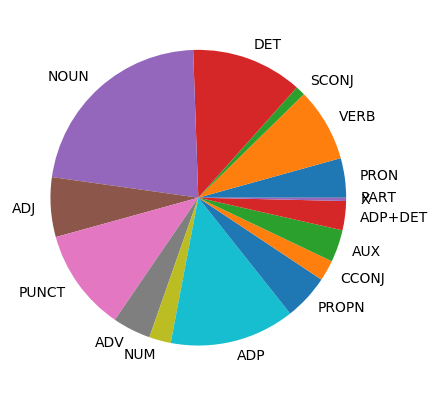
\includegraphics[width=.7\linewidth]{sequoiatest_img.png}
\caption{distribution des labels}
\end{minipage}
\end{figure} \subparagraph{Données de train \\ }  
 Nombre de phrases : 2231\\ 
\begin{figure}[H] \begin{minipage}{0.48\textwidth} \centering \begin{tabular}{|l || *{11 }{|c} |} \hline
Mot & Apparitions  \\ \hline
\begin{verb} de \end{verb} &2435\\ \hline
\begin{verb} , \end{verb} &2354\\ \hline
\begin{verb} . \end{verb} &1683\\ \hline
\begin{verb} la \end{verb} &1176\\ \hline
\begin{verb} __DIGIT__ \end{verb} &1039\\ \hline
\begin{verb} l' \end{verb} &916\\ \hline
\begin{verb} à \end{verb} &857\\ \hline
\begin{verb} et \end{verb} &845\\ \hline
\begin{verb} des \end{verb} &759\\ \hline
\begin{verb} le \end{verb} &743\\ \hline

\end{tabular}
\caption{ Mots les plus utilisés dans le set sequoia(train) } \label{Fig:muw}\end{minipage} 
\begin{minipage}{0.48\textwidth} \centering
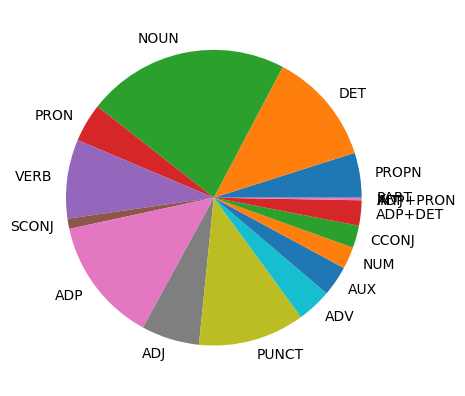
\includegraphics[width=.7\linewidth]{sequoiatrain_img.png}
\caption{distribution des labels}
\end{minipage}
\end{figure}


\clearpage \subsection{partut } 
 \begin{itemize} 
 \item[Présentation :] Ensemble varié de textes, incluant de extraits de conférences comme des extraits de Wikipedia ou des textes légaux

 \item[Pourcentage de mots hors vocabulaire : ]5.743
 \item[KL-Divergence :]0.330
 \end{itemize}  \subparagraph{Données de test \\ }  
 Nombre de phrases : 110\\ 
\begin{figure}[H] \begin{minipage}{0.48\textwidth} \centering \begin{tabular}{|l || *{11 }{|c} |} \hline
Mot & Apparitions  \\ \hline
\begin{verb} de \end{verb} &120\\ \hline
\begin{verb} . \end{verb} &110\\ \hline
\begin{verb} , \end{verb} &79\\ \hline
\begin{verb} la \end{verb} &69\\ \hline
\begin{verb} à \end{verb} &58\\ \hline
\begin{verb} l' \end{verb} &56\\ \hline
\begin{verb} les \end{verb} &46\\ \hline
\begin{verb} et \end{verb} &42\\ \hline
\begin{verb} des \end{verb} &39\\ \hline
\begin{verb} le \end{verb} &39\\ \hline

\end{tabular}
\caption{ Mots les plus utilisés dans le set partut(test) } \label{Fig:muw}\end{minipage} 
\begin{minipage}{0.48\textwidth} \centering
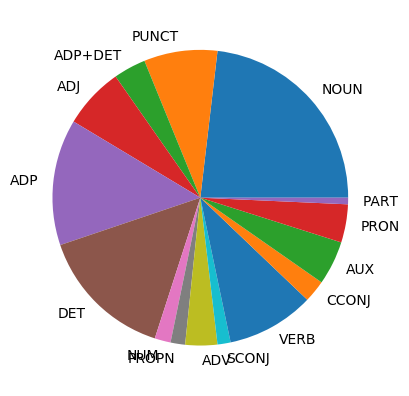
\includegraphics[width=.7\linewidth]{partuttest_img.png}
\caption{distribution des labels}
\end{minipage}
\end{figure} \subparagraph{Données de train \\ }  
 Nombre de phrases : 803\\ 
\begin{figure}[H] \begin{minipage}{0.48\textwidth} \centering \begin{tabular}{|l || *{11 }{|c} |} \hline
Mot & Apparitions  \\ \hline
\begin{verb} de \end{verb} &1114\\ \hline
\begin{verb} , \end{verb} &1016\\ \hline
\begin{verb} . \end{verb} &750\\ \hline
\begin{verb} la \end{verb} &683\\ \hline
\begin{verb} et \end{verb} &544\\ \hline
\begin{verb} l' \end{verb} &486\\ \hline
\begin{verb} des \end{verb} &432\\ \hline
\begin{verb} à \end{verb} &404\\ \hline
\begin{verb} d' \end{verb} &397\\ \hline
\begin{verb} le \end{verb} &385\\ \hline

\end{tabular}
\caption{ Mots les plus utilisés dans le set partut(train) } \label{Fig:muw}\end{minipage} 
\begin{minipage}{0.48\textwidth} \centering
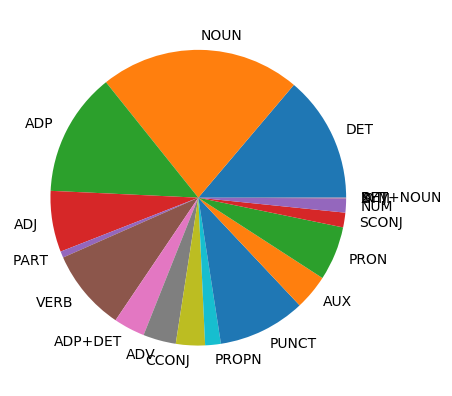
\includegraphics[width=.7\linewidth]{partuttrain_img.png}
\caption{distribution des labels}
\end{minipage}
\end{figure}


\clearpage \subsection{gsd } 
 \begin{itemize} 
 \item[Présentation :] Phrases variées

 \item[Pourcentage de mots hors vocabulaire : ]1.359
 \item[KL-Divergence :]0.409
 \end{itemize}  \subparagraph{Données de test \\ }  
 Nombre de phrases : 416\\ 
\begin{figure}[H] \begin{minipage}{0.48\textwidth} \centering \begin{tabular}{|l || *{11 }{|c} |} \hline
Mot & Apparitions  \\ \hline
\begin{verb} , \end{verb} &489\\ \hline
\begin{verb} de \end{verb} &426\\ \hline
\begin{verb} . \end{verb} &353\\ \hline
\begin{verb} la \end{verb} &222\\ \hline
\begin{verb} et \end{verb} &182\\ \hline
\begin{verb} l' \end{verb} &171\\ \hline
\begin{verb} à \end{verb} &168\\ \hline
\begin{verb} __DIGIT__ \end{verb} &166\\ \hline
\begin{verb} le \end{verb} &155\\ \hline
\begin{verb} les \end{verb} &127\\ \hline

\end{tabular}
\caption{ Mots les plus utilisés dans le set gsd(test) } \label{Fig:muw}\end{minipage} 
\begin{minipage}{0.48\textwidth} \centering
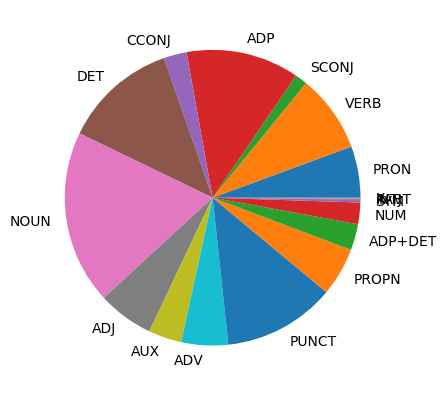
\includegraphics[width=.7\linewidth]{gsdtest_img.png}
\caption{distribution des labels}
\end{minipage}
\end{figure} \subparagraph{Données de train \\ }  
 Nombre de phrases : 14450\\ 
\begin{figure}[H] \begin{minipage}{0.48\textwidth} \centering \begin{tabular}{|l || *{11 }{|c} |} \hline
Mot & Apparitions  \\ \hline
\begin{verb} de \end{verb} &16964\\ \hline
\begin{verb} , \end{verb} &16595\\ \hline
\begin{verb} . \end{verb} &13359\\ \hline
\begin{verb} la \end{verb} &8676\\ \hline
\begin{verb} et \end{verb} &7148\\ \hline
\begin{verb} __DIGIT__ \end{verb} &7095\\ \hline
\begin{verb} le \end{verb} &6389\\ \hline
\begin{verb} à \end{verb} &6216\\ \hline
\begin{verb} l' \end{verb} &5864\\ \hline
\begin{verb} en \end{verb} &4793\\ \hline

\end{tabular}
\caption{ Mots les plus utilisés dans le set gsd(train) } \label{Fig:muw}\end{minipage} 
\begin{minipage}{0.48\textwidth} \centering
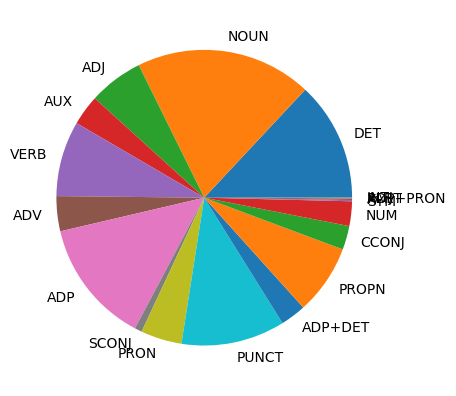
\includegraphics[width=.7\linewidth]{gsdtrain_img.png}
\caption{distribution des labels}
\end{minipage}
\end{figure}

\clearpage
\subsection{foot } 
 \begin{itemize} 
 \item[Présentation :] Ensemble de tweets parlant de football

 \end{itemize}  \subparagraph{Données de test \\ }  
 Nombre de phrases : 743\\ 
\begin{figure}[H] \begin{minipage}{0.48\textwidth} \centering \begin{tabular}{|l || *{11 }{|c} |} \hline
Mot & Apparitions  \\ \hline
\begin{verb} __MENTION__ \end{verb} &549\\ \hline
\begin{verb} la \end{verb} &433\\ \hline
\begin{verb} __SHARP__ \end{verb} &395\\ \hline
\begin{verb} Juventus \end{verb} &368\\ \hline
\begin{verb} : \end{verb} &338\\ \hline
\begin{verb} de \end{verb} &325\\ \hline
\begin{verb} ! \end{verb} &314\\ \hline
\begin{verb} le \end{verb} &257\\ \hline
\begin{verb} , \end{verb} &247\\ \hline
\begin{verb} __URL__ \end{verb} &226\\ \hline

\end{tabular}
\caption{ Mots les plus utilisés dans le set foot(test) } \label{Fig:muw}\end{minipage} 
\begin{minipage}{0.48\textwidth} \centering
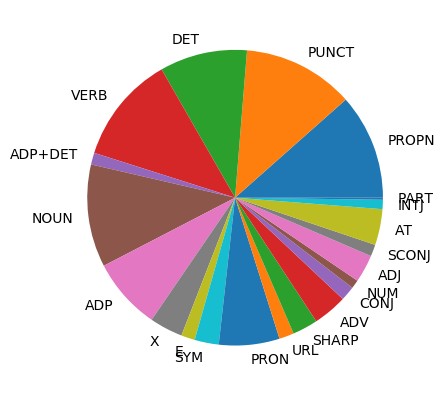
\includegraphics[width=.7\linewidth]{foottest_img.png}
\caption{distribution des labels}
\end{minipage}
\end{figure}


 \subsection{natdis } 
 \begin{itemize} 
 \item[Présentation :] Ensemble de tweets

 \end{itemize}  \subparagraph{Données de test \\ }  
 Nombre de phrases : 622\\ 
\begin{figure}[H] \begin{minipage}{0.48\textwidth} \centering \begin{tabular}{|l || *{11 }{|c} |} \hline
Mot & Apparitions  \\ \hline
\begin{verb} de \end{verb} &994\\ \hline
\begin{verb} __URL__ \end{verb} &469\\ \hline
\begin{verb} __DIGIT__ \end{verb} &411\\ \hline
\begin{verb} terre \end{verb} &338\\ \hline
\begin{verb} __SHARP__ \end{verb} &300\\ \hline
\begin{verb} tremblement \end{verb} &295\\ \hline
\begin{verb} : \end{verb} &285\\ \hline
\begin{verb} chaleur \end{verb} &244\\ \hline
\begin{verb} au \end{verb} &220\\ \hline
\begin{verb} vague \end{verb} &206\\ \hline

\end{tabular}
\caption{ Mots les plus utilisés dans le set natdis(test) } \label{Fig:muw}\end{minipage} 
\begin{minipage}{0.48\textwidth} \centering
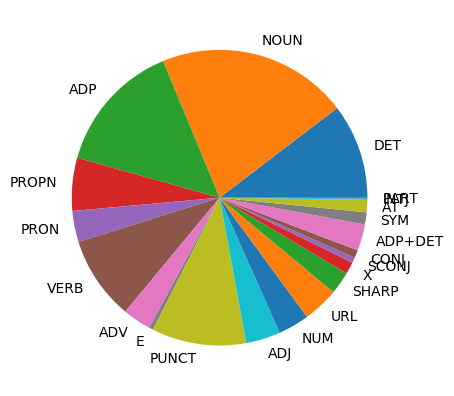
\includegraphics[width=.7\linewidth]{natdistest_img.png}
\caption{distribution des labels}
\end{minipage}
\end{figure}

\onehalfspacing



\section{Présentation du code}
Le code est regroupé dans les fichiers suivants:
\begin{description}
\item[helpers.py] Regroupe des fonctions utiles pour le chargement des
  données ou le test des résultats.
\item[tex\_data\_describe.py et tex\_result\_describe.py] Regroupe des fonctions
  utile pour (respectivement) décrire les données ou les
  résultats vers un ou plusieurs fichiers \LaTeX
\item[modele.py] fournit une interface commune aux différents
  classifieurs. 
\item[multiclass\_perceptron.py] Le perceptron multiclasse du TP5.
\item[modele\_tp5.py] Le perceptron utilisé avec les features du TP
  5.
\item[modele\_pj\_distrib.py] Inclut le modèle de perceptron
  implémenteant les 
  features proposées dans le sujet du projet, incluant les
  \emph{distributional features}.
\item[modele\_pj\_nodistrib.py] Même chose que modele\_pj\_distrib,
  sans les \emph{distributional features}
\item[modeles\_sklearn.py] Utilise deux implémentations de
  classifieurs provenant de la bibliothèque SKLearn.
\end{description}

\subsection{Description des classifieurs}
Les classifieurs possèdent tous la même interface, qui est indiquée
dans {\verb modele.py } \\ 
L'algorithme de classification utilisé pour tous les modèles (hors
ceux  provenant du
module {\verb modeles_sklearn } ) est le perceptron implémenté
dans {\verb multiclass_perceptron } Ainsi, seules les features sont
différentes. \\ Chaque feature est décrite en fonction de la
phrase $sentence$ , et du mot $w$ dont il faut prédire le label, qui
est situé à la position $pos$ dans la phrase. 
% TODO : mettre paragraph

\paragraph{} {\verb Modele_tp5 } 

Ce modèle implémente les features proposées lors du tp 5, qui sont les
suivantes : \\

\begin{itemize}
\item Le mot $w$
\item Les trois derniers caractères de $w$
\item Le premier caractère de $w$
\item Le dernier caractère de $w$
\item un booléen indiquant si le premier caractère est une lettre
  majuscule 
\item un booléen indiquant si tout le mot est écrit en majuscule
\item Le mot précédent dans la phrase
\item Le mot situé à $pos - 2$ dans la phrase.
\item Le mot suivant dans la phrase
\item Le mot situé à $pos + 2$ dans la phrase.
\end{itemize}

Ces features sont implémentées dans la fonction
{\verb build_sparse2 }, et le fichier contenant le Modele est
{\verb modele_tp5.py }.


\paragraph{} {\verb Modele_projet } et {\verb Modele_nodistrib } \\
Implémentent les features proposées dans le sujet du projet : 
\begin{itemize}
\item $w$ 
\item Les deux mots précédant est suivant $w$
\item Le nombre de mots avant $w$ dans la phrase
\item Le nombre de mots suivant $w$ dans la phrase
\item Un booléen indiquant si le mot se finit par un s
\item Un ensemble de booléens, indiquants respectivement si :
  \begin{itemize}
  \item le mot contient un chiffre
  \item le mot contient un tiret
  \item le mot est écrit en majuscules
  \item le mot se finit en {\verb -é }
  \item le mot se finit en {\verb -er }
  \item le mot se finit en {\verb -ant }
  \end{itemize}
\item les \emph{ distributional features }. Elles sont est composées de deux
  features, qu'on appellera respectivement ``distribution à
  droite'' et ``distribution à gauche''.\\
  Pour chaque mot $w$, on regarde le mot juste à droite $c$ (resp.juste à
  gauche), et on calcule le nombre de fois où le nombre de couples
  $w c$ (resp $c w$) apparaît dans le corpus de test. \\
  Les deux features sont égales à ce nombre. On se limite à calculer
  le nombre d'apparitions de ces couples pour $c$ faisant partie des
  10 mots les plus utilisés.
\end{itemize}
La classe {\verb Modele_nodistrib } n'implémente pas les \emph{
  distributional features}. \\
Les deux classes se trouvent respectivement dans
{\verb modele_pj_distrib } et {\verb modele_ph_nodistrib }

\paragraph{} {\verb Modele_sklearn_Perceptron } et {\verb Modele_SKLearn_SVM }
\\
Les features sont construites à partir des informations suivantes :
\begin{itemize}
\item $w$
\item un booléen indiquant si $w$ est écrit en lettres majuscules
\item un booléen indiquant si $w$ commence par une lettre majuscule
\item les trois dernières lettres du mot
\item les deux dernières lettres du mot
\item les trois premières lettres du mot
\item Le mot précédent
\item Le mot suivant
\item un booléen indiquant si le mot est un nombre
\item un booléen indiquant si le mot contient des lettres majuscules  
\end{itemize}

Le dictionnaire représentant les features est donné à une instance de
la classe {\verb DictVectorizer }, qui ``transformera'' ces features
en une forme acceptable pour le classifieur. Ensuite, la
classification sera réalisée par une instance de {\verb Perceptron} ou
  de {\verb LinearSVC }.



  

  


\section{Résultats}

\section{Résultats}
Dans un premier temps, voici les résultats des modèles sur le
dataset {\verb ftb }

 \begin{figure}[H] ·\centering \begin{tabular}{ |l|| *{5}{c|} }\hline
Classifieur   & Modele tp5 & Perceptron nodistrib & Perceptron distrib & SKLearn Perceptron & SKLearn SVM \\ \hline Pourcentage de réussite   & 94.70 & 93.97 & 93.47 & 94.13 & 96.71 \\ \hline  \end{tabular} \caption{Taux de réussite sur les données pour divers clasifieurs} \end{figure}



Nous remarquons que :
\begin{itemize}
\item Les résultats sont bons sur cet ensemble de données (avec
  plus de 90 \% à chaque fois.
  Cela reste à relativiser, étant donné que ces données d'entraînement sont
  de loin les plus conséquentes, avec plus de 14000 phrases.
\item La construction du dictionnaire nécessaire aux
  \emph{distributional features} prend beaucoup de temps.
\item Les \emph{distributional features} que l'on a construit
  ne servent à rien; au contraire elles baissent le score de réussite sur
  le \emph{dataset} {\verb ftb }.
  Cela est probablement dû à une mauvais compréhension de l'article,
  ayant mené à une mauvaise implémentation.
\end{itemize}

Maintenant, nous allons nous intéresser à des tableaux de résultats
plus détaillés. Pour chacun de ces tableaux, chaque colonne représente
un ensemble d'entraînement, tandis que chaque ligne représente un
ensemble de test. 


Pour chaque ensemble d'entraînement de de test, nous avons trois
mesures, toutes exprimées en pourcentage :
\begin{description}
\item[OOV] La réussite sur les mots hors vocabulaire, ie les mots
  apparaissant dans l'ensemble de test mais pas dans l'ensemble
  d'entrainement.
\item[AMB] La réussite sur les mots ambigus, qui apparaissent dans les
  données de train ou de test, et qui peuvent avoir deux natures
  différentes
\item[GEN] Le taux de réussite général.
\end{description}

\begin{figure}[H] \begin{adjustbox}{width=\textwidth} \begin{centering} \begin{tabular}{ | l || *{ 6}{c|c|c||} } \hline 
& \multicolumn{3}{|c|}{ ftb } & \multicolumn{3}{|c|}{ gsd } & \multicolumn{3}{|c|}{ partut } & \multicolumn{3}{|c|}{ pud } & \multicolumn{3}{|c|}{ sequoia } & \multicolumn{3}{|c|}{ spoken }  \\ \hline 
& OOV & AMB & GEN & OOV & AMB & GEN & OOV & AMB & GEN & OOV & AMB & GEN & OOV & AMB & GEN & OOV & AMB & GEN   \\ \hline \hline 
foot  & 25.46 & 82.28 & 65.95
 & 22.34 & 77.01 & 67.94
 & 42.11 & 73.30 & 61.04
 & 42.11 & 73.30 & 61.04
 & 33.37 & 78.45 & 64.89
 & 31.63 & 69.44 & 50.65
 \\ \hline 
ftb  & 76.31 & 93.01 & 94.70
 & 70.97 & 90.93 & 91.01
 & 69.94 & 86.36 & 85.29
 & 69.94 & 86.36 & 85.29
 & 76.85 & 91.23 & 90.36
 & 44.26 & 71.82 & 62.65
 \\ \hline 
gsd  & 67.61 & 89.03 & 89.99
 & 78.81 & 93.51 & 94.62
 & 69.04 & 88.87 & 85.36
 & 69.04 & 88.87 & 85.36
 & 76.96 & 91.59 & 90.02
 & 45.01 & 75.84 & 64.46
 \\ \hline 
natdis  & 24.92 & 87.98 & 78.52
 & 46.93 & 86.72 & 79.10
 & 51.74 & 78.38 & 71.35
 & 51.74 & 78.38 & 71.35
 & 51.72 & 84.71 & 76.22
 & 31.10 & 69.26 & 55.00
 \\ \hline 
partut  & 74.03 & 87.81 & 90.81
 & 71.73 & 92.37 & 91.84
 & 69.28 & 90.81 & 91.13
 & 69.28 & 90.81 & 91.13
 & 79.17 & 92.70 & 90.13
 & 50.87 & 75.71 & 69.22
 \\ \hline 
pud  & 61.45 & 81.50 & 84.84
 & 67.53 & 84.02 & 87.96
 & 67.81 & 79.07 & 80.64
 & 67.81 & 79.07 & 80.64
 & 72.38 & 80.88 & 83.76
 & 47.75 & 75.58 & 64.63
 \\ \hline 
sequoia  & 70.82 & 90.18 & 91.06
 & 73.17 & 93.20 & 92.73
 & 70.61 & 90.15 & 85.69
 & 70.61 & 90.15 & 85.69
 & 81.31 & 94.37 & 94.64
 & 46.44 & 75.60 & 65.06
 \\ \hline 
spoken  & 49.55 & 71.92 & 78.64
 & 51.09 & 77.00 & 82.50
 & 60.32 & 75.70 & 76.85
 & 60.32 & 75.70 & 76.85
 & 63.71 & 73.80 & 78.02
 & 78.57 & 86.65 & 90.34
 \\ \hline 
 \end{tabular} \end{centering} \end{adjustbox} \caption{ Taux de réussite détaillés pour le perceptron Modele tp5} \end{figure} 

De manière générale, le score de 90\% sur la réussite des données
était flatteur, la plupart des résultats tournant autour de 80\%

Nous remarquons que les scores les plus bas sur les tests
proviennent des ensembles de test natdis et foot
(resp. autour de 80 et 70 \% sur la plupart des corpus).


Deux explications pourraient exister : La première étant que, de
manière générale, les tweets sont rarement écrits dans un français
correct,
la seconde serait que ces derniers contiennent
un grand nombre de labels spécifiques
(par exemple les mentions) à twitter.


Par conséquent, des scores particulièrement bas sur ces \emph{dataset}
se retrouveront avec les autres classifieurs.


\begin{figure}[H] \begin{adjustbox}{width=\textwidth} \begin{centering} \begin{tabular}{ | l || *{ 6}{c|c|c||} } \hline 
& \multicolumn{3}{|c|}{ ftb } & \multicolumn{3}{|c|}{ gsd } & \multicolumn{3}{|c|}{ partut } & \multicolumn{3}{|c|}{ pud } & \multicolumn{3}{|c|}{ sequoia } & \multicolumn{3}{|c|}{ spoken }  \\ \hline 
& OOV & AMB & GEN & OOV & AMB & GEN & OOV & AMB & GEN & OOV & AMB & GEN & OOV & AMB & GEN & OOV & AMB & GEN   \\ \hline \hline 
foot  & 12.98 & 79.61 & 59.18
 & 18.69 & 76.62 & 63.53
 & 18.90 & 76.33 & 46.63
 & 18.90 & 76.33 & 46.63
 & 21.33 & 78.00 & 57.85
 & 20.39 & 72.79 & 43.13
 \\ \hline 
ftb  & 61.13 & 92.70 & 93.47
 & 62.01 & 90.52 & 89.05
 & 51.37 & 84.32 & 75.70
 & 51.37 & 84.32 & 75.70
 & 58.72 & 90.26 & 83.50
 & 33.64 & 73.98 & 55.87
 \\ \hline 
gsd  & 47.98 & 89.35 & 87.30
 & 65.97 & 92.43 & 91.93
 & 46.12 & 85.90 & 75.09
 & 46.12 & 85.90 & 75.09
 & 56.81 & 89.96 & 82.50
 & 33.08 & 76.76 & 57.20
 \\ \hline 
natdis  & 16.68 & 86.56 & 75.15
 & 36.73 & 85.83 & 75.97
 & 28.52 & 78.70 & 57.04
 & 28.52 & 78.70 & 57.04
 & 34.05 & 86.82 & 66.93
 & 23.25 & 74.80 & 50.05
 \\ \hline 
partut  & 56.73 & 89.89 & 89.78
 & 58.69 & 89.98 & 88.07
 & 49.82 & 86.08 & 81.55
 & 49.82 & 86.08 & 81.55
 & 57.72 & 90.70 & 80.79
 & 38.49 & 75.71 & 61.15
 \\ \hline 
pud  & 41.10 & 80.53 & 81.12
 & 55.42 & 83.10 & 85.25
 & 45.70 & 79.59 & 70.91
 & 45.70 & 79.59 & 70.91
 & 51.88 & 80.47 & 76.15
 & 34.36 & 78.40 & 57.09
 \\ \hline 
sequoia  & 54.20 & 91.51 & 88.81
 & 59.69 & 92.32 & 89.77
 & 45.03 & 86.12 & 74.57
 & 45.03 & 86.12 & 74.57
 & 60.51 & 92.48 & 88.03
 & 34.75 & 76.94 & 57.51
 \\ \hline 
spoken  & 36.09 & 71.55 & 76.28
 & 33.71 & 76.72 & 79.42
 & 35.75 & 73.76 & 65.82
 & 35.75 & 73.76 & 65.82
 & 44.16 & 72.65 & 70.95
 & 57.03 & 85.13 & 83.21
 \\ \hline 
 \end{tabular} \end{centering} \end{adjustbox} \caption{ Taux de réussite détaillés pour le perceptron Perceptron distrib} \end{figure} 
\begin{figure}[H] \begin{adjustbox}{width=\textwidth} \begin{centering} \begin{tabular}{ | l || *{ 6}{c|c|c||} } \hline 
& \multicolumn{3}{|c|}{ ftb } & \multicolumn{3}{|c|}{ gsd } & \multicolumn{3}{|c|}{ partut } & \multicolumn{3}{|c|}{ pud } & \multicolumn{3}{|c|}{ sequoia } & \multicolumn{3}{|c|}{ spoken }  \\ \hline 
& OOV & AMB & GEN & OOV & AMB & GEN & OOV & AMB & GEN & OOV & AMB & GEN & OOV & AMB & GEN & OOV & AMB & GEN   \\ \hline \hline 
foot  & 13.45 & 81.01 & 58.36
 & 14.70 & 74.18 & 58.75
 & 16.12 & 64.02 & 40.47
 & 16.12 & 64.02 & 40.47
 & 17.18 & 68.54 & 48.65
 & 15.21 & 69.78 & 37.44
 \\ \hline 
ftb  & 56.30 & 90.86 & 90.45
 & 57.78 & 88.05 & 86.13
 & 46.65 & 75.54 & 69.89
 & 46.65 & 75.54 & 69.89
 & 54.40 & 87.40 & 80.11
 & 29.77 & 70.88 & 51.73
 \\ \hline 
gsd  & 42.52 & 86.02 & 83.07
 & 58.15 & 90.30 & 88.68
 & 43.75 & 75.74 & 68.74
 & 43.75 & 75.74 & 68.74
 & 47.40 & 86.65 & 77.03
 & 27.81 & 74.51 & 52.22
 \\ \hline 
natdis  & 19.68 & 85.66 & 72.86
 & 34.20 & 83.68 & 72.67
 & 22.25 & 71.88 & 50.77
 & 22.25 & 71.88 & 50.77
 & 35.61 & 82.30 & 63.01
 & 18.34 & 68.89 & 43.26
 \\ \hline 
partut  & 63.46 & 84.55 & 85.68
 & 40.21 & 89.27 & 85.12
 & 49.48 & 78.24 & 75.26
 & 49.48 & 78.24 & 75.26
 & 56.46 & 87.41 & 79.52
 & 32.88 & 73.81 & 56.93
 \\ \hline 
pud  & 34.53 & 80.95 & 78.66
 & 48.81 & 81.08 & 82.09
 & 42.35 & 70.28 & 65.20
 & 42.35 & 70.28 & 65.20
 & 45.75 & 78.37 & 72.14
 & 29.38 & 75.14 & 52.20
 \\ \hline 
sequoia  & 51.03 & 88.47 & 85.07
 & 54.12 & 90.18 & 86.41
 & 41.58 & 78.22 & 68.71
 & 41.58 & 78.22 & 68.71
 & 53.94 & 89.11 & 83.42
 & 29.61 & 74.42 & 52.75
 \\ \hline 
spoken  & 35.98 & 70.89 & 72.15
 & 31.40 & 74.11 & 75.81
 & 35.67 & 64.43 & 59.84
 & 35.67 & 64.43 & 59.84
 & 40.53 & 68.96 & 65.40
 & 49.74 & 80.71 & 76.75
 \\ \hline 
 \end{tabular} \end{centering} \end{adjustbox} \caption{ Taux de réussite détaillés pour le perceptron Perceptron nodistrib} \end{figure} 
Nous remarquons que la plus grosse différence entre les deux consiste
en le score de réussite dans la classification
des mots hors vocabulaire, mais aussi et surtout que le score général 
des mots hors-vocabulaire est très bas par rapport aux autres
classifieurs, dont celui du TP5 \\
Etant donné que toutes les features du TP5 sont présentes dans ce
perceptron, l'explication la plus logique est que les features
ajoutées ne sont pas utiles, et que par conséquent en ajoutant ces
features on complexifie les calculs, ce qui cause cette baisse de la
précision , spécifiqument sur les calculs des mots hors vocabulaire.
\\
Cela est montré par le fait que le perception possédant les
\emph{distributional features} est légèrement moins précis, notamment
sur les mots hors vocabulaire. \\

\begin{figure}[H] \begin{adjustbox}{width=\textwidth} \begin{centering} \begin{tabular}{ | l || *{ 6}{c|c|c||} } \hline 
& \multicolumn{3}{|c|}{ ftb } & \multicolumn{3}{|c|}{ gsd } & \multicolumn{3}{|c|}{ partut } & \multicolumn{3}{|c|}{ pud } & \multicolumn{3}{|c|}{ sequoia } & \multicolumn{3}{|c|}{ spoken }  \\ \hline 
& OOV & AMB & GEN & OOV & AMB & GEN & OOV & AMB & GEN & OOV & AMB & GEN & OOV & AMB & GEN & OOV & AMB & GEN   \\ \hline \hline 
foot  & 33.39 & 78.41 & 67.50
 & 22.68 & 76.55 & 68.47
 & 35.72 & 74.06 & 56.63
 & 35.72 & 74.06 & 56.63
 & 30.69 & 80.58 & 65.61
 & 43.07 & 71.03 & 57.42
 \\ \hline 
ftb  & 74.17 & 91.38 & 94.13
 & 76.99 & 88.72 & 90.89
 & 66.69 & 87.56 & 85.34
 & 66.69 & 87.56 & 85.34
 & 73.49 & 89.68 & 90.02
 & 51.32 & 73.40 & 66.45
 \\ \hline 
gsd  & 67.06 & 86.07 & 88.95
 & 81.07 & 91.52 & 94.23
 & 68.01 & 89.22 & 85.64
 & 68.01 & 89.22 & 85.64
 & 72.79 & 90.68 & 89.69
 & 52.39 & 76.40 & 67.92
 \\ \hline 
natdis  & 23.71 & 84.23 & 77.32
 & 29.57 & 84.79 & 75.75
 & 46.81 & 82.26 & 68.55
 & 46.81 & 82.26 & 68.55
 & 47.40 & 83.04 & 74.63
 & 39.65 & 76.16 & 60.66
 \\ \hline 
partut  & 72.11 & 86.06 & 90.09
 & 73.91 & 90.60 & 90.69
 & 64.84 & 91.75 & 91.96
 & 64.84 & 91.75 & 91.96
 & 74.44 & 90.70 & 89.38
 & 51.45 & 74.38 & 69.34
 \\ \hline 
pud  & 57.61 & 79.01 & 83.57
 & 69.22 & 82.05 & 87.52
 & 63.33 & 78.32 & 79.83
 & 63.33 & 78.32 & 79.83
 & 67.68 & 79.92 & 83.21
 & 50.98 & 76.92 & 66.44
 \\ \hline 
sequoia  & 71.21 & 88.30 & 90.63
 & 75.84 & 90.99 & 92.49
 & 69.14 & 90.62 & 86.17
 & 69.14 & 90.62 & 86.17
 & 77.53 & 93.17 & 94.68
 & 51.87 & 76.88 & 67.82
 \\ \hline 
spoken  & 51.10 & 68.74 & 77.67
 & 48.26 & 75.71 & 82.27
 & 60.32 & 74.82 & 77.24
 & 60.32 & 74.82 & 77.24
 & 59.58 & 72.82 & 78.74
 & 73.97 & 83.31 & 89.31
 \\ \hline 
 \end{tabular} \end{centering} \end{adjustbox} \caption{ Taux de réussite détaillés pour le perceptron SKLearn Perceptron} \end{figure} 

Ici, les résultats sont légèrement meilleurs que le perceptron du
TP5. Cela est plausiblement dû soit à une meilleure implémentation de
l'algorithme (ou une meilleure extraction des features avec
{\verb DictVectorizer } ).
ou à un nombre d'epoch plus élevé. 


L'amélioration la plus sensible par rapport au TP5
est le meilleur score sur les mots
hors-vocabulaire. 
\\

\begin{figure}[H] \begin{adjustbox}{width=\textwidth} \begin{centering} \begin{tabular}{ | l || *{ 6}{c|c|c||} } \hline 
& \multicolumn{3}{|c|}{ ftb } & \multicolumn{3}{|c|}{ gsd } & \multicolumn{3}{|c|}{ partut } & \multicolumn{3}{|c|}{ pud } & \multicolumn{3}{|c|}{ sequoia } & \multicolumn{3}{|c|}{ spoken }  \\ \hline 
& OOV & AMB & GEN & OOV & AMB & GEN & OOV & AMB & GEN & OOV & AMB & GEN & OOV & AMB & GEN & OOV & AMB & GEN   \\ \hline \hline 
foot  & 36.30 & 83.83 & 70.94
 & 23.19 & 79.04 & 70.02
 & 38.49 & 75.80 & 61.56
 & 38.49 & 75.80 & 61.56
 & 33.59 & 82.43 & 67.77
 & 30.08 & 74.43 & 51.53
 \\ \hline 
ftb  & 83.78 & 95.06 & 96.71
 & 80.84 & 91.87 & 92.91
 & 76.79 & 89.63 & 89.38
 & 76.79 & 89.63 & 89.38
 & 79.38 & 92.08 & 92.52
 & 44.66 & 76.24 & 64.92
 \\ \hline 
gsd  & 73.93 & 90.46 & 92.16
 & 85.06 & 94.59 & 96.16
 & 77.35 & 90.92 & 89.55
 & 77.35 & 90.92 & 89.55
 & 78.46 & 92.75 & 92.25
 & 47.49 & 79.27 & 67.43
 \\ \hline 
natdis  & 25.36 & 88.78 & 80.16
 & 43.58 & 87.86 & 79.65
 & 51.51 & 83.22 & 73.80
 & 51.51 & 83.22 & 73.80
 & 50.88 & 85.10 & 77.10
 & 30.18 & 81.49 & 57.16
 \\ \hline 
partut  & 85.57 & 91.15 & 93.71
 & 77.17 & 93.26 & 92.92
 & 75.76 & 94.72 & 95.06
 & 75.76 & 94.72 & 95.06
 & 82.64 & 92.47 & 91.92
 & 51.83 & 76.85 & 71.05
 \\ \hline 
pud  & 63.01 & 82.10 & 86.08
 & 69.06 & 84.31 & 88.90
 & 71.48 & 79.61 & 83.47
 & 71.48 & 79.61 & 83.47
 & 72.09 & 81.61 & 85.46
 & 48.04 & 79.47 & 66.65
 \\ \hline 
sequoia  & 78.73 & 92.61 & 93.90
 & 78.04 & 94.75 & 94.66
 & 75.93 & 92.71 & 89.46
 & 75.93 & 92.71 & 89.46
 & 82.75 & 95.22 & 96.39
 & 48.85 & 78.55 & 67.62
 \\ \hline 
spoken  & 54.74 & 74.08 & 81.35
 & 51.22 & 79.55 & 84.67
 & 63.80 & 78.14 & 80.50
 & 63.80 & 78.14 & 80.50
 & 66.89 & 78.20 & 83.32
 & 81.54 & 89.09 & 92.88
 \\ \hline 
 \end{tabular} \end{centering} \end{adjustbox} \caption{ Taux de réussite détaillés pour le perceptron SKLearn SVM} \end{figure} 

Nous notons des performances légèrement meilleures partout pour le SVM
que pour le Perceptron (l'implémentation de SKLearn), malgré le même
set de features.

Cela est logique, puisque le premier est un
algorithme plus évolué que le second, qui par conséquent permet une
meilleure précision.




%%%  
%D'après nos résultats, nos modèles ont un résultat pratiquement
%similaire avec seulement 3\%  de différence entre le plus mauvais modèles, 
%Perceptron nodistrib, et le meilleur, SKLearn SVM.
%Nous remarquons par ailleurs les modèles perdent du résultats en
%majeur partis à cause du  corpus foot, 
%en effet le corpus foot ne possède que très peu de vocabulaires
%similaires aux autres corpus dû à 
%son vocabulaire spécifique avec en moyenne moins de 40\% de
%vocabulaire reconnus.  Ce qui permet d'avoir des résultats à peine
%bons avec une moyenne  générale des modèles autours des 60\%
%seulement. Quant à natdis , notre second corpus sans trains, il
%possède aussi un vocabulaire  spécifique puisque moins de 50\% du
%vocabulaire dans le test   est reconnus. Cependant, il possède de
%meilleurs résultats généraux  que foot avec une moyenne autour des
%70\%. On peut en déduire  que le vocabulaire spécifique est
%généralement peu retrouvé et   donc que l'OOV et les résultats sont en
%corrélation, en effet  lorsque l'on regarde d'autres résultats comme
%spoken.train  et sequoia.test avec un OOV de 40\% en moyenne,
%le résultat n'est autour que des 60\% pour les modèles les moins bons. 
 

 \begin{figure}[H] ·\centering \begin{tabular}{ |l|| *{5}{c|} }\hline
Classifieur   & Modele tp5 & Perceptron nodistrib & Perceptron distrib & SKLearn Perceptron & SKLearn SVM \\ \hline Pourcentage de réussite   & 94.70 & 93.97 & 93.47 & 94.13 & 96.71 \\ \hline  \end{tabular} \caption{Taux de réussite sur les données pour divers clasifieurs} \end{figure}
\begin{figure}[H] \begin{adjustbox}{width=\textwidth} \begin{centering} \begin{tabular}{ | l || *{ 6}{c|c|c||} } \hline 
& \multicolumn{3}{|c|}{ ftb } & \multicolumn{3}{|c|}{ gsd } & \multicolumn{3}{|c|}{ partut } & \multicolumn{3}{|c|}{ pud } & \multicolumn{3}{|c|}{ sequoia } & \multicolumn{3}{|c|}{ spoken }  \\ \hline 
& OOV & AMB & GEN & OOV & AMB & GEN & OOV & AMB & GEN & OOV & AMB & GEN & OOV & AMB & GEN & OOV & AMB & GEN   \\ \hline \hline 
foot  & 22.59 & 80.79 & 62.63
 & 22.22 & 73.40 & 64.74
 & 34.42 & 54.63 & 52.56
 & 34.42 & 54.63 & 52.56
 & 25.72 & 66.45 & 55.48
 & 27.65 & 70.13 & 46.27
 \\ \hline 
ftb  & 72.59 & 91.46 & 92.68
 & 72.65 & 88.20 & 88.76
 & 61.63 & 70.21 & 75.75
 & 61.63 & 70.21 & 75.75
 & 66.23 & 86.56 & 83.22
 & 35.81 & 70.89 & 55.14
 \\ \hline 
gsd  & 66.30 & 86.74 & 87.80
 & 79.51 & 89.87 & 91.60
 & 59.11 & 73.77 & 75.92
 & 59.11 & 73.77 & 75.92
 & 64.67 & 84.70 & 81.58
 & 36.56 & 74.00 & 56.92
 \\ \hline 
natdis  & 24.25 & 87.42 & 76.99
 & 39.30 & 85.03 & 76.20
 & 41.62 & 71.63 & 62.23
 & 41.62 & 71.63 & 62.23
 & 38.50 & 81.83 & 67.66
 & 22.28 & 75.64 & 48.98
 \\ \hline 
partut  & 71.15 & 87.56 & 88.66
 & 64.13 & 89.98 & 88.42
 & 62.11 & 73.64 & 79.56
 & 62.11 & 73.64 & 79.56
 & 68.76 & 86.0 & 81.39
 & 41.48 & 74.19 & 61.07
 \\ \hline 
pud  & 58.28 & 81.36 & 83.36
 & 69.32 & 81.76 & 85.86
 & 59.18 & 65.35 & 71.88
 & 59.18 & 65.35 & 71.88
 & 63.58 & 77.23 & 77.47
 & 40.57 & 75.02 & 58.29
 \\ \hline 
sequoia  & 68.74 & 89.43 & 89.53
 & 72.59 & 90.56 & 90.70
 & 61.19 & 75.90 & 76.44
 & 61.19 & 75.90 & 76.44
 & 67.85 & 88.33 & 86.57
 & 38.93 & 73.47 & 57.38
 \\ \hline 
spoken  & 45.03 & 70.93 & 75.45
 & 45.68 & 72.81 & 77.75
 & 50.0 & 61.08 & 65.96
 & 50.0 & 61.08 & 65.96
 & 48.07 & 64.16 & 65.23
 & 65.22 & 81.94 & 81.24
 \\ \hline 
 \end{tabular} \end{centering} \end{adjustbox} \caption{ taux de réussite} \end{figure} 
\begin{figure}[H] \begin{adjustbox}{width=\textwidth} \begin{centering} \begin{tabular}{ | l || *{ 6}{c|c|c||} } \hline 
& \multicolumn{3}{|c|}{ ftb } & \multicolumn{3}{|c|}{ gsd } & \multicolumn{3}{|c|}{ partut } & \multicolumn{3}{|c|}{ pud } & \multicolumn{3}{|c|}{ sequoia } & \multicolumn{3}{|c|}{ spoken }  \\ \hline 
& OOV & AMB & GEN & OOV & AMB & GEN & OOV & AMB & GEN & OOV & AMB & GEN & OOV & AMB & GEN & OOV & AMB & GEN   \\ \hline \hline 
foot  & 13.47 & 80.21 & 58.29
 & 13.71 & 74.31 & 58.93
 & 14.60 & 67.05 & 38.91
 & 14.60 & 67.05 & 38.91
 & 18.35 & 69.62 & 50.86
 & 12.84 & 70.73 & 36.64
 \\ \hline 
ftb  & 57.25 & 90.61 & 90.62
 & 54.09 & 88.13 & 85.70
 & 45.02 & 79.49 & 70.04
 & 45.02 & 79.49 & 70.04
 & 57.30 & 88.14 & 80.99
 & 26.35 & 71.93 & 49.89
 \\ \hline 
gsd  & 44.92 & 86.04 & 83.73
 & 53.99 & 90.25 & 88.23
 & 40.80 & 81.26 & 69.16
 & 40.80 & 81.26 & 69.16
 & 49.33 & 87.75 & 77.87
 & 24.71 & 74.97 & 50.72
 \\ \hline 
natdis  & 19.37 & 84.76 & 72.73
 & 32.50 & 84.97 & 73.67
 & 21.33 & 76.79 & 49.79
 & 21.33 & 76.79 & 49.79
 & 37.48 & 83.17 & 65.19
 & 15.51 & 73.34 & 41.80
 \\ \hline 
partut  & 57.69 & 84.72 & 86.44
 & 38.04 & 87.76 & 84.01
 & 49.48 & 85.0 & 75.70
 & 49.48 & 85.0 & 75.70
 & 54.57 & 88.11 & 79.52
 & 30.65 & 74.57 & 54.87
 \\ \hline 
pud  & 35.91 & 80.44 & 78.99
 & 47.38 & 81.61 & 81.72
 & 38.22 & 74.45 & 64.49
 & 38.22 & 74.45 & 64.49
 & 47.70 & 78.99 & 73.20
 & 27.12 & 76.38 & 51.08
 \\ \hline 
sequoia  & 53.70 & 88.82 & 86.19
 & 53.42 & 91.08 & 86.37
 & 38.68 & 82.37 & 68.17
 & 38.68 & 82.37 & 68.17
 & 53.94 & 89.65 & 83.42
 & 26.41 & 74.98 & 51.14
 \\ \hline 
spoken  & 35.20 & 70.98 & 72.92
 & 30.24 & 73.40 & 75.42
 & 28.31 & 68.34 & 58.92
 & 28.31 & 68.34 & 58.92
 & 41.95 & 69.77 & 66.45
 & 43.29 & 80.79 & 74.94
 \\ \hline 
 \end{tabular} \end{centering} \end{adjustbox} \caption{ Pourcentage de réussite du classifieur courant} \end{figure} 
\begin{figure}[H] \begin{adjustbox}{width=\textwidth} \begin{centering} \begin{tabular}{ | l || *{ 6}{c|c|c||} } \hline 
& \multicolumn{3}{|c|}{ ftb } & \multicolumn{3}{|c|}{ gsd } & \multicolumn{3}{|c|}{ partut } & \multicolumn{3}{|c|}{ pud } & \multicolumn{3}{|c|}{ sequoia } & \multicolumn{3}{|c|}{ spoken }  \\ \hline 
& OOV & AMB & GEN & OOV & AMB & GEN & OOV & AMB & GEN & OOV & AMB & GEN & OOV & AMB & GEN & OOV & AMB & GEN   \\ \hline \hline 
foot  & 14.37 & 80.23 & 57.75
 & 14.95 & 74.20 & 59.46
 & 17.32 & 73.26 & 42.60
 & 17.32 & 73.26 & 42.60
 & 15.44 & 67.25 & 46.71
 & 13.93 & 64.54 & 35.78
 \\ \hline 
ftb  & 57.33 & 90.74 & 90.42
 & 58.03 & 87.98 & 86.25
 & 51.32 & 82.50 & 73.40
 & 51.32 & 82.50 & 73.40
 & 55.33 & 86.96 & 80.09
 & 29.42 & 68.89 & 50.58
 \\ \hline 
gsd  & 46.01 & 86.41 & 83.86
 & 59.20 & 90.37 & 89.37
 & 47.18 & 84.35 & 72.50
 & 47.18 & 84.35 & 72.50
 & 48.63 & 86.23 & 76.65
 & 26.80 & 71.44 & 50.56
 \\ \hline 
natdis  & 19.64 & 84.88 & 72.24
 & 34.46 & 84.62 & 73.20
 & 26.30 & 79.71 & 53.43
 & 26.30 & 79.71 & 53.43
 & 39.06 & 80.80 & 63.80
 & 18.32 & 67.69 & 44.00
 \\ \hline 
partut  & 57.69 & 85.47 & 86.36
 & 40.21 & 89.27 & 84.89
 & 54.26 & 86.89 & 79.68
 & 54.26 & 86.89 & 79.68
 & 58.67 & 88.82 & 80.11
 & 34.81 & 69.25 & 54.51
 \\ \hline 
pud  & 37.90 & 80.49 & 79.07
 & 48.28 & 82.36 & 82.67
 & 45.19 & 76.09 & 68.41
 & 45.19 & 76.09 & 68.41
 & 45.79 & 77.63 & 71.91
 & 29.13 & 72.80 & 51.23
 \\ \hline 
sequoia  & 52.02 & 89.24 & 85.77
 & 55.16 & 90.11 & 86.48
 & 44.59 & 84.92 & 72.22
 & 44.59 & 84.92 & 72.22
 & 52.50 & 89.90 & 83.30
 & 28.47 & 72.02 & 51.12
 \\ \hline 
spoken  & 34.76 & 70.36 & 71.55
 & 29.85 & 73.23 & 75.43
 & 35.80 & 71.35 & 62.23
 & 35.80 & 71.35 & 62.23
 & 41.21 & 66.75 & 63.19
 & 48.28 & 77.75 & 74.22
 \\ \hline 
 \end{tabular} \end{centering} \end{adjustbox} \caption{ taux de réussite} \end{figure} 


\section{Conclusion}
\end{document}
